\chapter{Matlab Verification}


\section{Introduction}

Conventional sigma-delta modulators are commonly used for performing A/D conversion in several sensor read-out applications, such as automotive, consumer electronics, medical instrumentation, environmental measurements, or even live audio recording from a microphone \cite{ESSCIRC_GUINEA}. However, these ADCs, which exhibit very high Dynamic Range (DR) thanks to oversampling and noise shaping techniques, typically feature a narrower bandwidth with respect to Nyquist rate ADCs.

Moreover, because of the memory effect inherent in sigma-delta modulation (each digital output sample somehow depends on the value of previous samples), they are not suitable for applications where single-shot events or multiple input sources with multiplexing must be evaluated.
Incremental ADCs (IADCs) overcome this limitation, since they are reset at the beginning of each conversion cycle \cite{PRIME_CAVALLO}. However, in IADCs high-resolution is obtained at the expense of a large number of clock cycles per conversion, preventing their use when relatively large bandwidth or short conversion time (latency) is required.

This shortcoming of IADCs can be overcome by exploiting the extended-range technique \cite{JSSC_CHEN}\cite{ISSCC_KIM}\cite{PRIME_MOATAZ}\cite{ICICDT_CAVALLO}\cite{ISVC_AGAH}, which allows the resolution to be increased while maintaining the conversion time relatively short. Extended-range architectures, however, are more susceptible than conventional IADCs to building-block non-idealities, which have then to be considered carefully. This paper provides some insight on the effect of operational amplifier (op-amp) specifications on extended-range IADC performance, in order to allow proper choice of the design parameters. 

\section{Extended-Range Incremental ADC}

An extended-range IADC is basically a two-stage A/D converter, in which the residue of the first-stage conversion, performed by a conventional IADC, is further digitized by a second stage (ERADC). The selection of the resolution required in each of the two stages to achieve a given overall effective number of bits (ENOB) affects the conversion time and, hence, the bandwidth of the overall ADC, as well as the requirements of the building blocks.

\begin{figure}
    \centering
    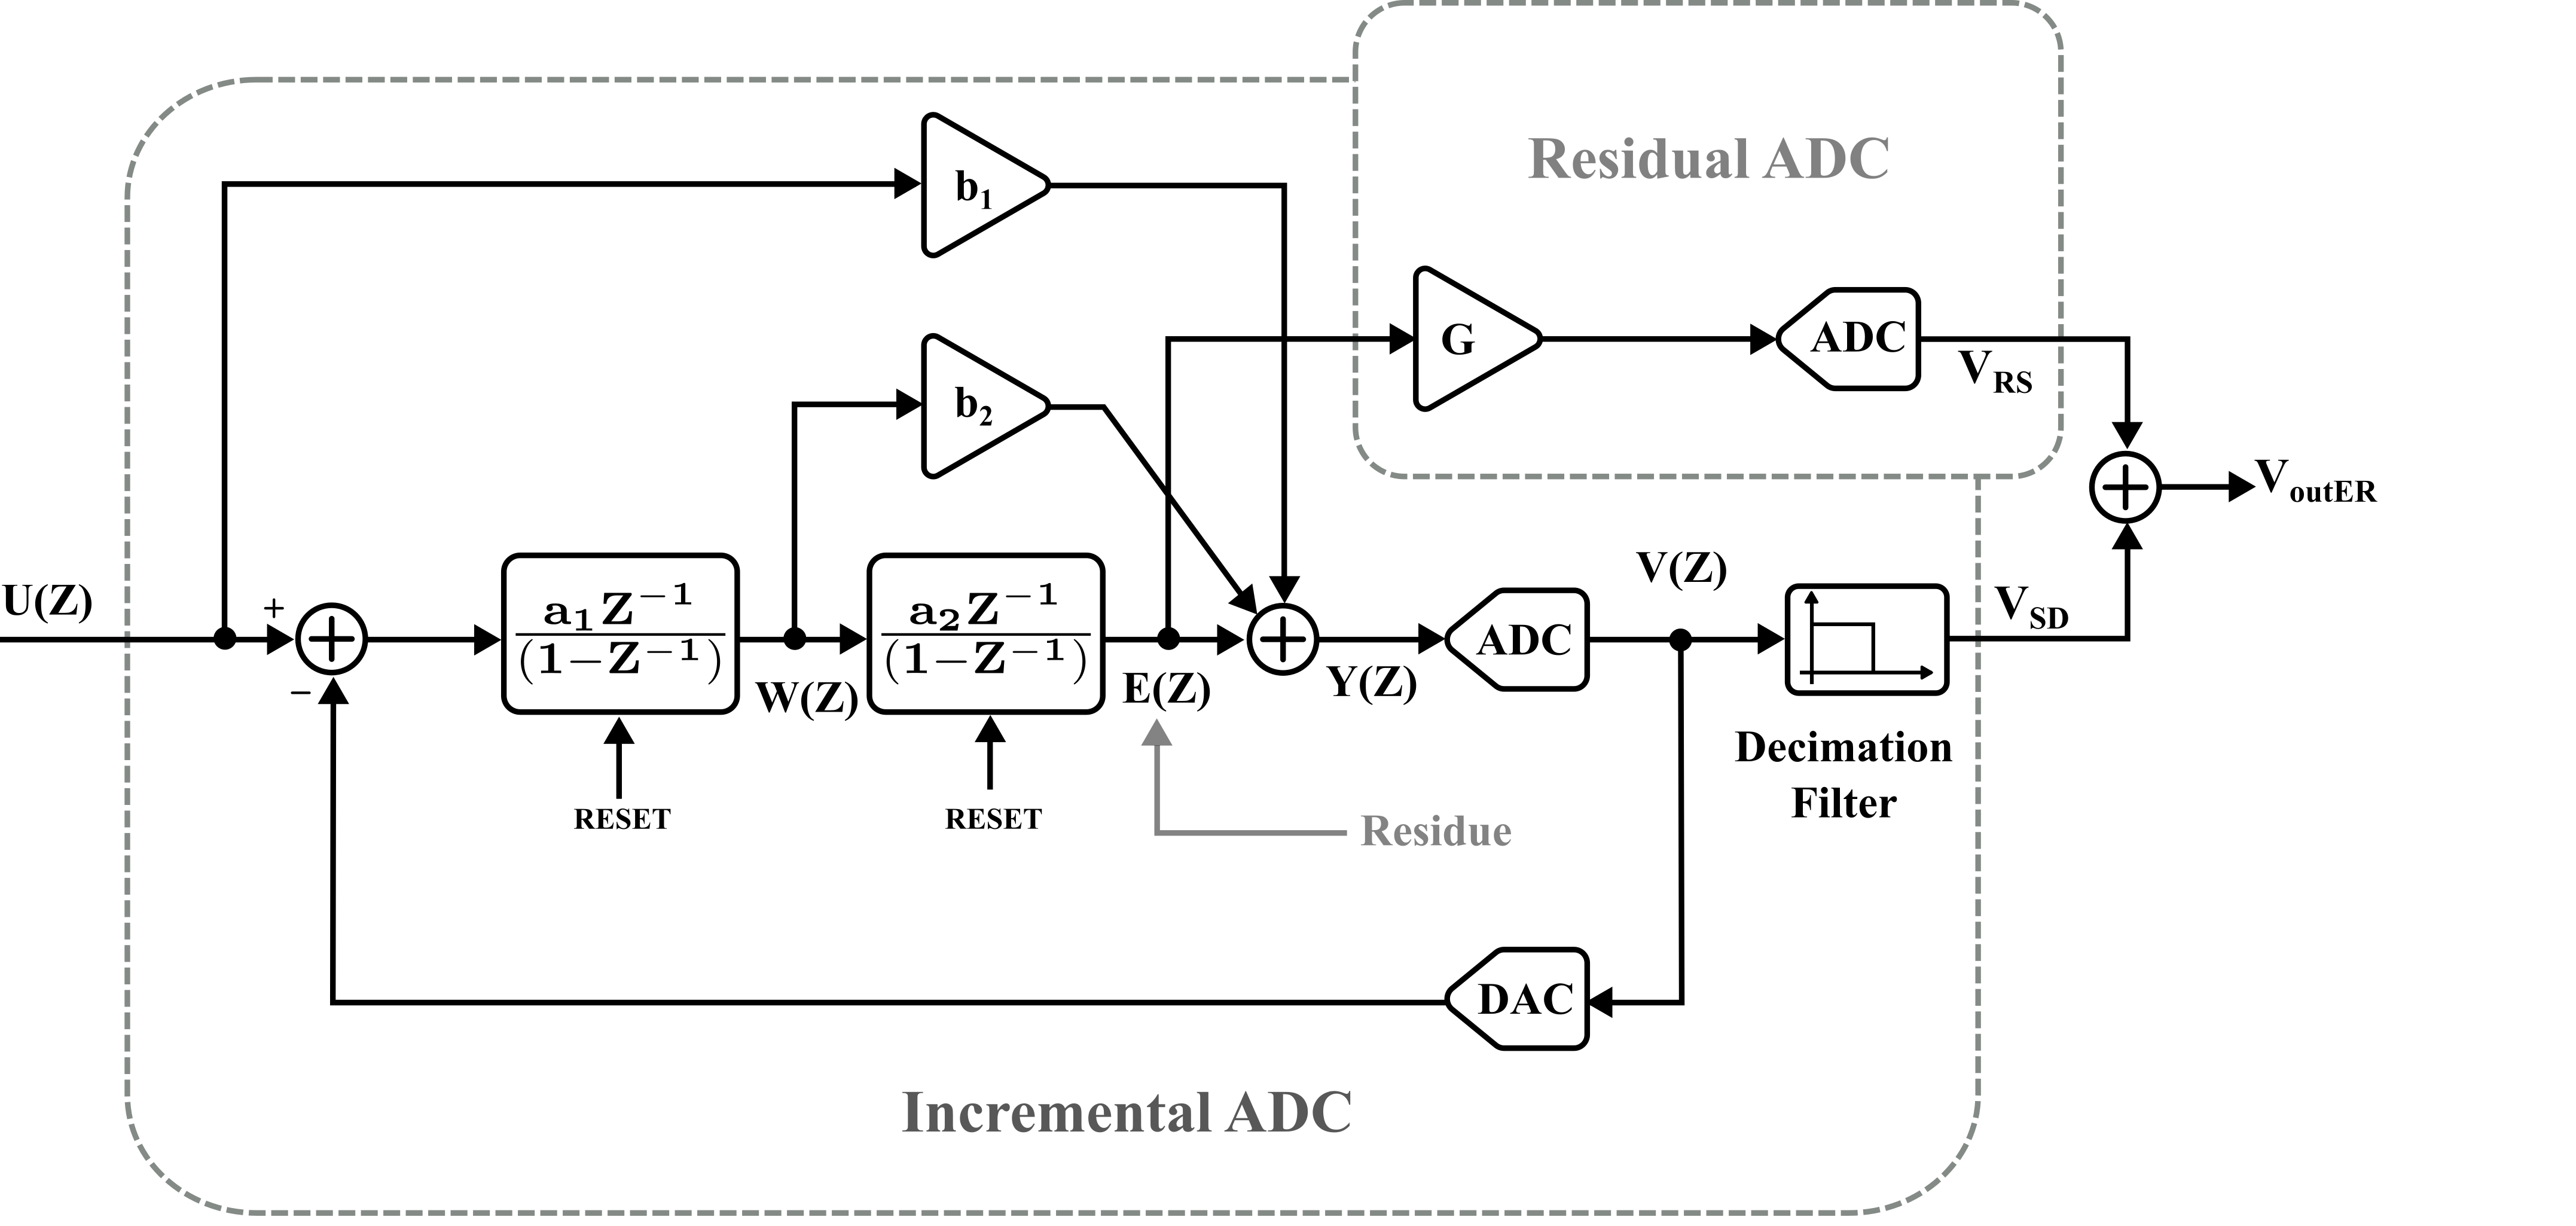
\includegraphics[width=\columnwidth]{extndd_range_scnd_ordr_sdm_ff_arch_adc_dac.png}
    \caption{Extended-range second-order feed-forward incremental ADC architecture}
    \label{ERISDM_MFF}
\end{figure}

The block diagram of the extended-range second-order IADC considered in this paper is shown in Fig. \ref{ERISDM_MFF}. The first stage of the ADC is a second-order IADC, consisting of two integrators, a multi-bit quantizer, a feedback DAC and decimation filter, while second stage consists of a gain block and the extended-range ADC (ERADC), which converts into the digital domain the residue of the first-stage conversion.

The IADC is reset at the beginning of each conversion cycle to clear all of the analog and digital memory elements. If the input signal amplitude is less than or equal to the Maximum Stable Amplitude (MSA) and if the poles of the noise transfer function (NTF) of the IADC loop are well within the unit circle, i.~e. the system is stable, then quantizer input $y$ remains bounded.

\subsection{Important Equations}

If the IADC runs for $i$ clock cycles, then the non-iterative expression of the signal at the input of the quantizer is

\begin{equation}
\begin{split}
    y[i]&=b_1u+b_2w[i]+a_1a_2u\sum_{j=1}^{i} (j-1)\\
        &-a_1a_2V_{ref}\sum_{j=1}^{i}\sum_{k=1}^{j-1} v[k-1]
\end{split}
\end{equation}

The value of $y$ at the end of the conversion, i.~e. after $M$ clock cycles, is given by
\begin{equation}
    \begin{split}
        y[M]&=b_1u+b_2w[M]+a_1a_2\frac{M(M-1)}{2}u\\
            &-a_1a_2V_{ref}\left(v[M-2]+.....+(M-1)v[0]\right)
    \end{split}
\end{equation}

Since the terms $y[M]$ and $w[M]$ are negligible, the reconstruction of the input signal sample $u$ is attainable from the $(M-2)$ output codes of the IADC. Provided that the oversampling ratio $M$ is large enough, the terms $y[M]$ and $w[M]$ become indeed insignificant with respect to the term $a_1a_2V_{ref}(v[M-2] + .... + (M-1)v[0])$ and reconstruction can be achieved by passing the IADC digital output signal through a decimation filter with down-sampling factor of $M$, according to
\begin{equation}\small\label{Vout_isdm}
\begin{split}
    V_{SD}&=\frac{2a_1a_2}{2b_1+a_1a_2M(M-1)}\\
                &\times V_{ref}\left(v[M-2]+.....+(M-1)v[0]\right)
\end{split}
\end{equation}
where $V_{SD}$ represents the closest digital equivalent of the input sample.
For multi-bit quantizer, considering a second-order loop filter with oversampling ratio of $M$, the obtainable effective number of bits (ENOB) can be expressed approximately as,
\begin{equation}
    ENOB_{IADC}\approx N_{SD}+2\log_{2}⁡(M)-2
\end{equation}
Where, $N_{SD}$ is the resolution of the IADC quantizer, $ENOB_{IADC}$ is the ENOB for IADC and $M$ is the oversampling ratio. The residue of the conversion is inherently available at the end of the conversion at the output of the second integrator and it is provided to the ERADC through gain block with gain of $G=2^{\left(N_{SD}-1\right)}$ for digitization. If the digitized input signal and digitized residue are added, then the overall output can be expressed as 
\begin{equation}\label{Vout_erisdm}
\begin{split}
V_{outER}=&V_{RS} + \\
          & +\frac{2a_1a_2}{2b_1+a_1a_2M(M-1)}V_{ref}\left(v[M-2] +\\
          & +...+(M-1)v[0]\right)
\end{split}
\end{equation}
From \eqref{Vout_erisdm} it can be observed that the addition of the digitized residue to the digitized input signal brings the overall digital signal $V_{outER}$ closer to the input signal, improving the signal-to-noise ratio by an amount equal to the dynamic range of the ERADC. Consequently, overall effective number of bits can be expressed as
\begin{equation}
    ENOB_{TOT}\approx N_{RS}+N_{SD}+2\log_{2}⁡(M)-2
\end{equation}
where $N_{RS}$ is the resolution of the ERADC, $N_{SD}$ is the resolution of the IADC quantizer and $M$ is the oversampling ratio.\\

\subsection{Conversion Timing}
The selection of the ERADC architecture and resolution is guided by the overall resolution requirement and the number of clock cycles available for the conversion.
\begin{figure}
    \centering
    
\includegraphics[width=\columnwidth]{timing_diagram.png}
    \caption{Conversion timing in an extended-range IADC}
    \label{TIMIG}
\end{figure}
 The conversion timing of an extended-range IADC is shown in Fig. \ref{TIMIG}. The first-stage IADC produces the digital output and the residue after $M$ clock cycles ($T_{SD}$). The residue is then applied to the ERADC for further digitization. The ERADC needs a time period $T_{RS}$ for the conversion, depending on the architecture employed. Therefore, the overall conversion time required turns out to be $T_{TOT}=T_{SD}+T_{RS}$.

 %%%%%%%%%%%%%%%%%%%%%%%%%%%%%%%%%%%%%%%%%%%%%%%%%%%%%%%%%%%%%%%%%%%%%%%%%%%%%%%%%%%%%%%%
\section{Analysis of Op-Amp Requirements}
 %%%%%%%%%%%%%%%%%%%%%%%%%%%%%%%%%%%%%%%%%%%%%%%%%%%%%%%%%%%%%%%%%%%%%%%%%%%%%%%%%%%%%%%%
Different combinations of resolution in IADC with a given value of $M$ and ERADC can fulfill a specific ENOB requirement. However, the sensitivity of each combination to the op-amp non-idealities varies, while selection of the optimum solution is necessary for robust performance. Therefore, the analysis of the op-amp specifications plays a very important role in selecting the best combination. The effects of op-amp non-idealities, such as gain and gain-bandwidth product (GBW), are, therefore, determined for an extended-range IADC with the combinations of resolution in IADC and ERADC summarized in Tab.~\ref{PARAM}, using a Simulink model.
\begin{table}
\centering
\begin{tabular}{c|c|c|c|c|c|c|c|c|c}
\Xhline{3\arrayrulewidth}
\textbf{ENOB\textsubscript{TOT}} & \multicolumn{3}{c|}{\textbf{12}} & \multicolumn{3}{c|}{\textbf{13}} & \multicolumn{3}{c}{\textbf{14}} \\ \hline
\textbf{N\textsubscript{SD}} & 3 & 3 & 4 & 3 & 3 & 4 & 3 & 3 & 4 \\ \hline
\textbf{ENOB\textsubscript{INC}} & 12 & 9 & 10 & 13 & 9 & 10 & 14 & 9 & 10 \\ \hline
\textbf{N\textsubscript{RS}} & 0 & 3 & 2 & 0 & 4 & 3 & 0 & 5 & 4 \\ \hline
\textbf{M} & 45 & 18 & 18 & 64 & 18 & 18 & 90 & 18 & 18 \\ \Xhline{3\arrayrulewidth}
\end{tabular}
\caption{Parameters of the considered extended-range IADC}
\label{PARAM}
\end{table}

\subsection{Effect of Low-Frequency Gain}
The first parameter to be considered is the low-frequency gain of the op-amps used in the first and second integrator of the second-order IADC. The variation of the gain affects the integrator coefficient, as well as the location of the integrator pole. In a stand-alone IADC, the shift in the location of the pole has more significant effect than the modification of the integrator coefficient, since the integrator pole sets the zero of the IADC NTF. However, in an extended-range IADC also the variation of the integrator coefficient becomes important, since it affects the value of the residue and can cause a degradation of the overall performance after recombination. The integrator transfer function considering finite op-amp low-frequency gain is given by \cite{TCAS_MALCOVATI} 
\begin{equation}
    H(Z)=\frac{C_s}{C_f}\frac{Z^{-1}}{1-\alpha Z^{-1}}
\end{equation}
Parameter $\alpha$ is given by
\begin{equation}
    \alpha\approx\frac{A_0C_f}{A_0C_f+C_s}
\end{equation}
%%%%%%%%%%%%%%%%%%%%%%%%%%%%%%%%%%%%%%%%%%%%%%%%%%%%%%%%%%%%%%%%%%%%%%%%%%%%%%%%%%%%%
%    NEW EQUATION
%%%%%%%%%%%%%%%%%%%%%%%%%%%%%%%%%%%%%%%%%%%%%%%%%%%%%%%%%%%%%%%%%%%%%%%%%%%%%%%%%%%%
and integrator coefficient `a' is given by
\begin{equation}
\begin{split}
    a &= \frac{A_0}{1+A_0\beta}\\
      &= \frac{A_0}{1+A_0\left(\frac{C_f}{C_s}\right)}
    \label{INTEG_COEFF}
\end{split}
\end{equation}
%%%%%%%%%%%%%%%%%%%%%%%%%%%%%%%%%%%%%%%%%%%%%%%%%%%%%%%%%%%%%%%%%%%%%%%%%%%%%%%%%%%%
where $C_s$ is the sampling capacitance, $C_f$ is the feedback capacitance and $A_0$ is the op-amp low frequency gain.

%%%%%%%%%%%%%%%%%%%%%%%%%%%%%%%%%%%%%%%%%%%%%%%%%%%%%%%%%%%%%%%%%%%%%%%%%%%%%%%%%%%%%
%   NEW PARAGRAPH
%%%%%%%%%%%%%%%%%%%%%%%%%%%%%%%%%%%%%%%%%%%%%%%%%%%%%%%%%%%%%%%%%%%%%%%%%%%%%%%%%%%%%
From Eq. \ref{INTEG_COEFF}, it is clear that, for ideal op-amp with infinite gain ($A_0=\infty$), the integrator coefficient is simply a ratio of $C_s$ and $C_f$. However, finite low-frequency gain modifies the coefficient degrading the output signal. Therefore in case of second order IADC, the residue, when passed through and processed by series of two integrators, gets corrupted. Nevertheless, since the point at which the residue is injected, is actually a point of injection of the quantization error, the change in the residue value would get high-pass filtered as quantization noise, the corrupted value should be in certain limit though. Extended-range IADC, however, rely on the accuracy of the residue signal, as it is the input to the second stage ADC. If the estimate of residue itself turns out to be inappropriate, it's digital equivalent will also get inaccurate degrading the overall response significantly. This implies that the variation of integrator coefficient has significant effect in extended-range IADC than in standalone IADC.
%%%%%%%%%%%%%%%%%%%%%%%%%%%%%%%%%%%%%%%%%%%%%%%%%%%%%%%%%%%%%%%%%%%%%%%%%%%%%%%%%%%%%
\subsubsection{Low-Frequency Gain of the First-Integrator Op-Amp}
The low-frequency gain of the first integrator op-amp in the IADC is varied from 0~dB to 100~dB considering the IADC standalone and extended-range architectures with the parameters shown in Table \ref{PARAM}. In Fig. \ref{SNR_G1}, the achieved SNR is plotted as a function of the op-amp gain for ENOB requirement of 12, 13 and 14 bits, respectively.
\begin{figure}
\centering
\subfloat[]{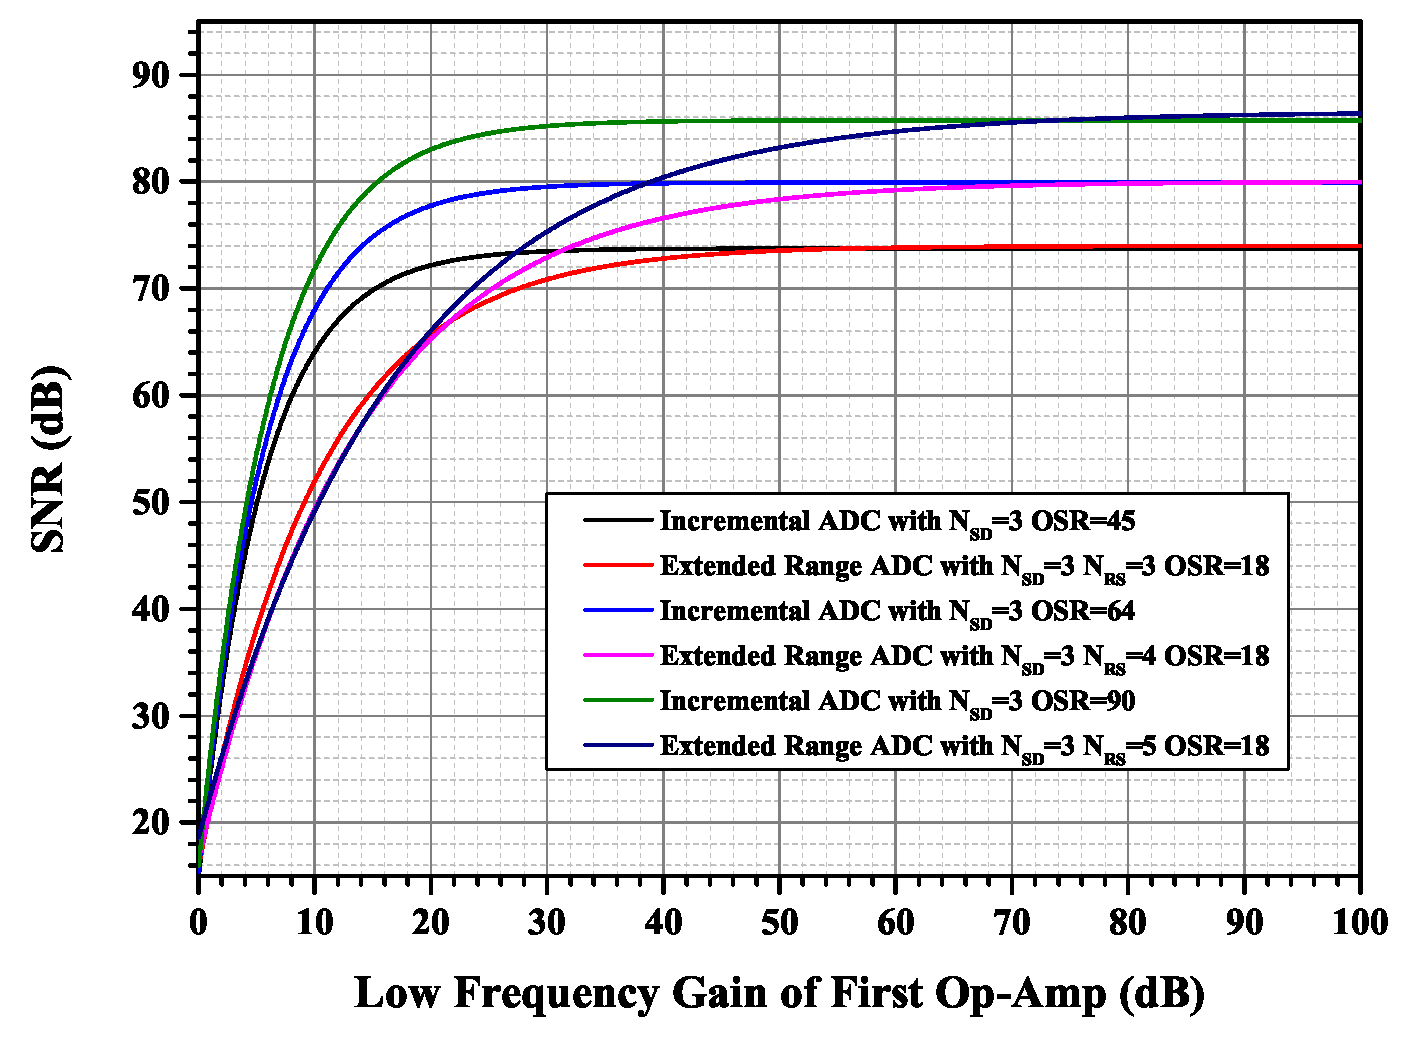
\includegraphics[width=2.5in]{Chap_paper01/Figures/SNR_G1_NSD3.eps}%
\label{SNR_G1_NSD3}}
\hfil
\subfloat[]{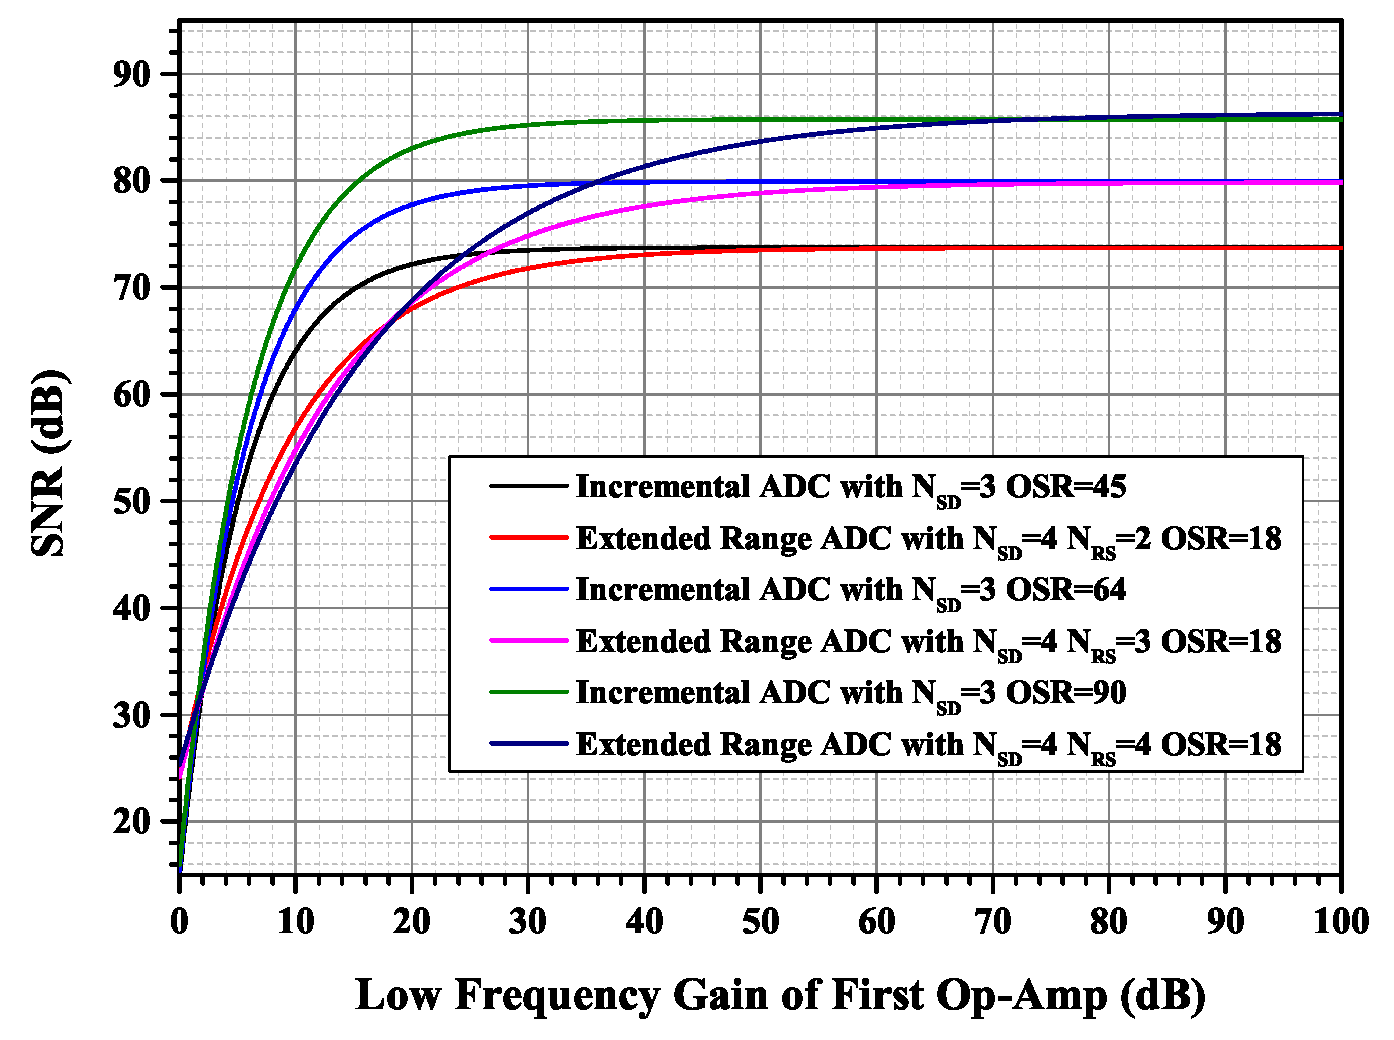
\includegraphics[width=2.5in]{Chap_paper01/Figures/SNR_G1_NSD4.eps}%
\label{SNR_G1_NSD4}}
\caption{Comparison of the IADC and extended-range IADC with different values of the first-integrator op-amp gain}
\label{SNR_G1}
\end{figure}
It can be observed that for the standalone IADC, the gain requirement is low and almost equal for all the three ENOB values, while in case of extended range IADC the gain requirement is considerably higher and increases as the ENOB requirement increases. The minimum gain needed for the IADC to achieve an SNR of 86~dB is around 40~dB, while that for the extended-range IADC it is around 70~dB. Obviously the conversion time for the extended-range IADC is much shorter than for the standalone IADC (less clock cycles are required).

\subsubsection{Low-Frequency Gain of the Second-Integrator Op-Amp}
The impact of the low-frequency gain of the second-integrator op-amp on the overall performance is negligible in standalone IADCs, but it turn out to be critical for extended-range IADCs, since it affects the integrator coefficient and, hence, the residue value. Fig. \ref{SNR_G2} shows this effect.
\begin{figure}
\centering
\subfloat[]{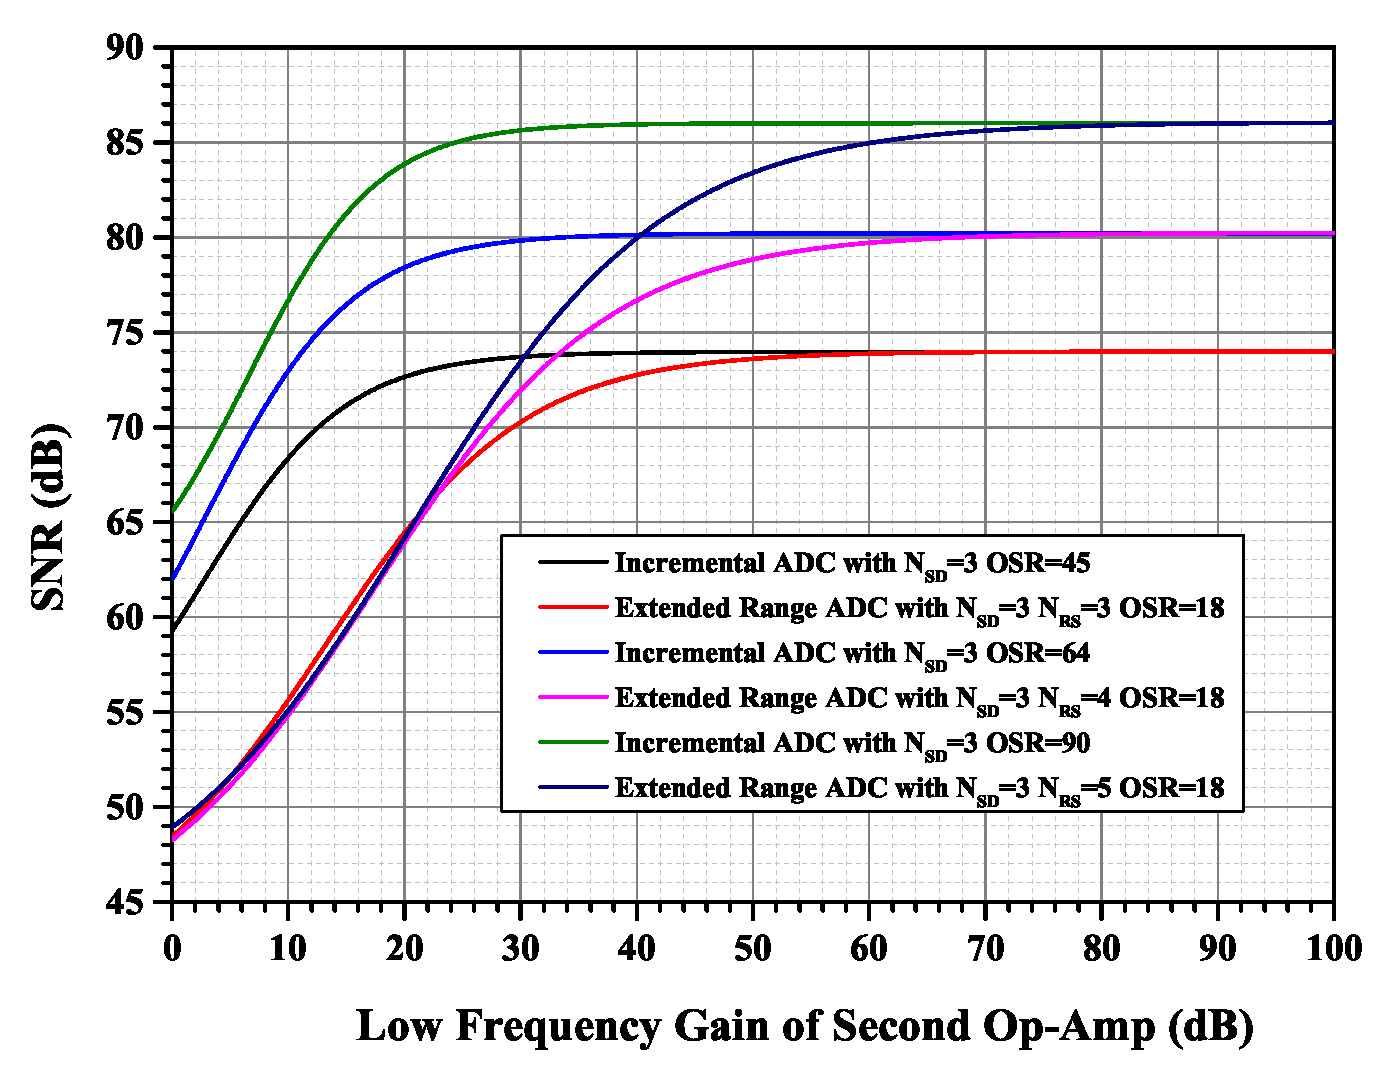
\includegraphics[width=2.5in]{Chap_paper01/Figures/SNR_G2_NSD3.eps}%
\label{SNR_G2_NSD3}}
\hfil
\subfloat[]{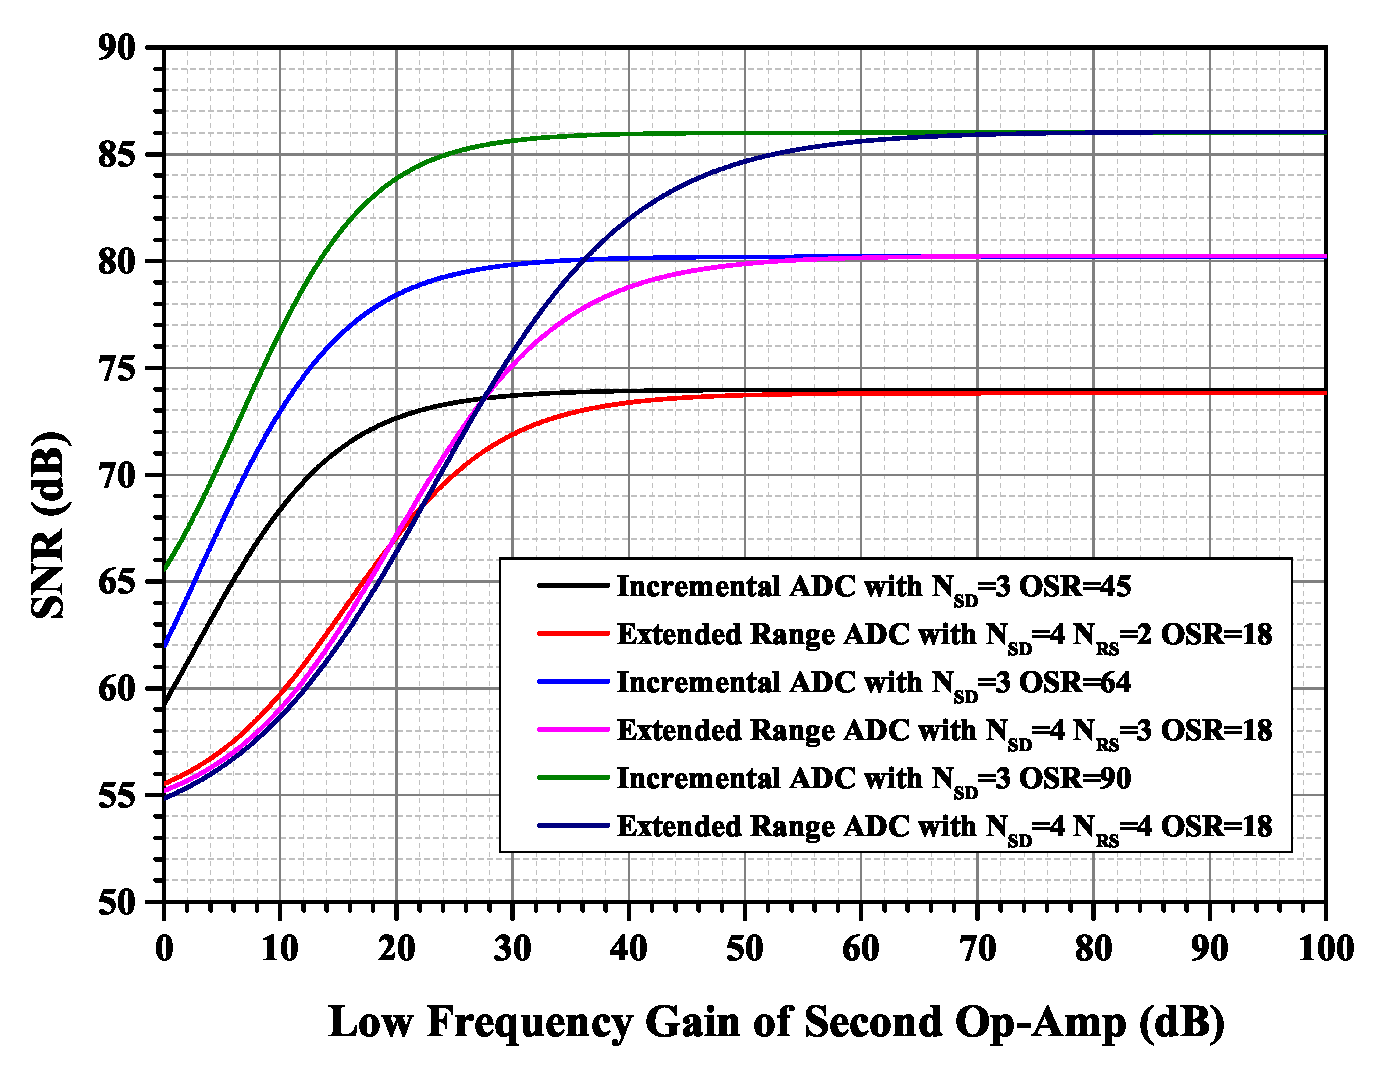
\includegraphics[width=2.5in]{Chap_paper01/Figures/SNR_G2_NSD4.eps}%
\label{SNR_G2_NSD4}}
\caption{Comparison of the IADC and extended-range IADC with different values of the second-integrator op-amp gain}
\label{SNR_G2}
\end{figure}

\subsection{Effect of Finite GBW of the Op-Amps}
Another major parameter which influences the ADC performance is the op-amp finite GBW. Finite GBW causes an incomplete charge transfer in the integrator at the end of each clock phase, leading to an error. A stand-alone IADC, is pretty robust against incomplete settling in the integrators. However, since the extended-range IADC performance relies on the accuracy of the residue value, which is obtained at the second integrator output, incomplete settling becomes quite detrimental for the overall ADC performance and, therefore, the op-amp GBW requirement becomes much more stringent. 
\subsubsection{GBW of the First-Integrator Op-Amp}
The performance of standalone IADC and extended-range IADC as a function of the first-integrator op-amp GBW is shown in Fig. \ref{SNR_GBW1}. Considering an ENOB requirement of 14 bits (SNR of 86~dB), the standalone IADC requires 60~MHz of GBW with a conversion time of 90 clock cycles, while the extended a conversion time of merely 18 clock cycles.
\begin{figure}
\centering
\subfloat[]{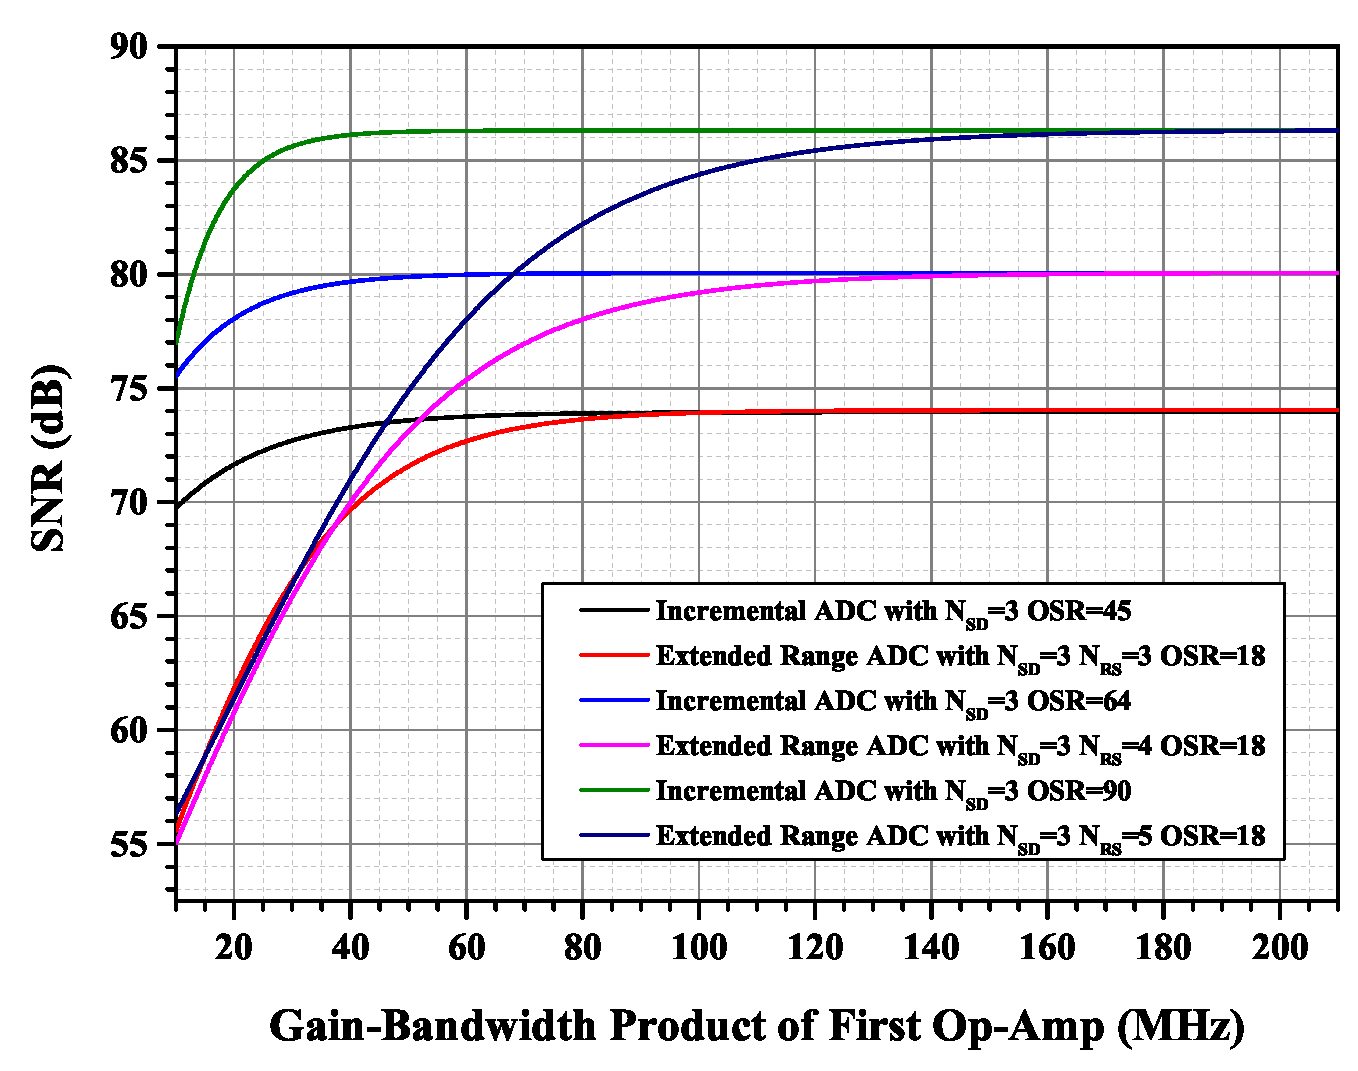
\includegraphics[width=2.5in]{Chap_paper01/Figures/SNR_GBW1_NSD3.eps}%
\label{SNR_GBW1_NSD3}}
\hfil
\subfloat[]{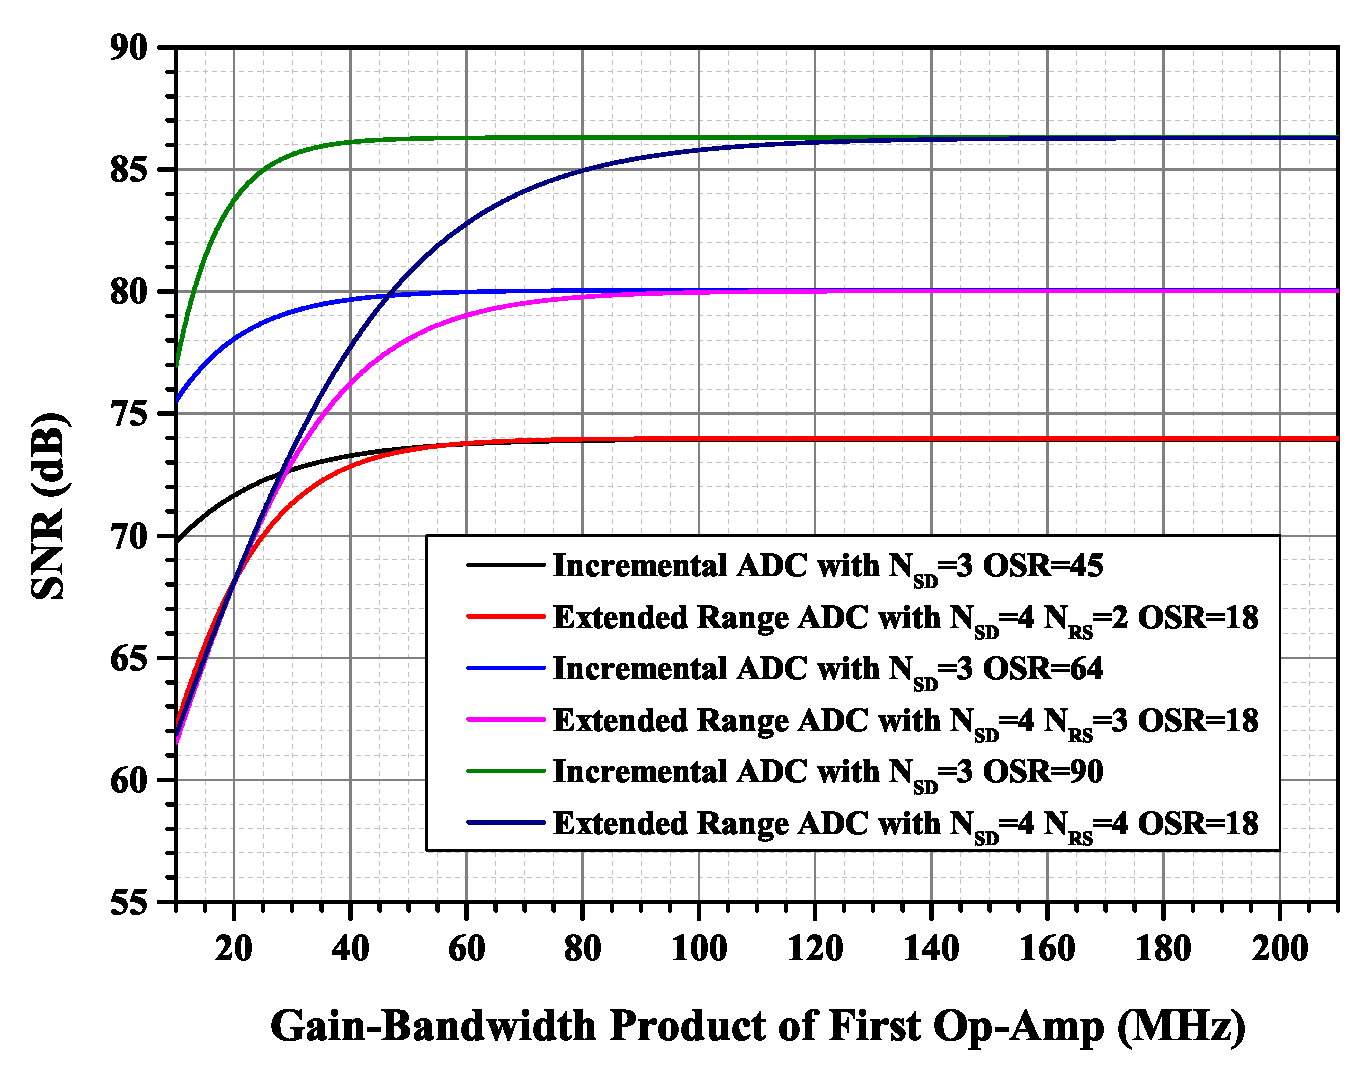
\includegraphics[width=2.5in]{Chap_paper01/Figures/SNR_GBW1_NSD4.eps}%
\label{SNR_GBW1_NSD4}}
\caption{Comparison of the IADC and extended-range IADC with different values of the first-integrator op-amp GBW}
\label{SNR_GBW1}
\end{figure}

\subsubsection{GBW of the Second-Integrator Op-Amp}
The second-integrator op-amp GBW has negligible effect on the performance of a standalone IADC, but again it affect the overall performance of extended-range IADCs, as shown in Fig. \ref{SNR_GBW2}. For an ENOB of 14 bits, the standalone IADC needs 40~MHz of GBW, while the extended-range IADC with $N_{INC}=9$ and $N_{RS}=5$ requires a GBW of 160~MHz.
\begin{figure}
\centering
\subfloat[]{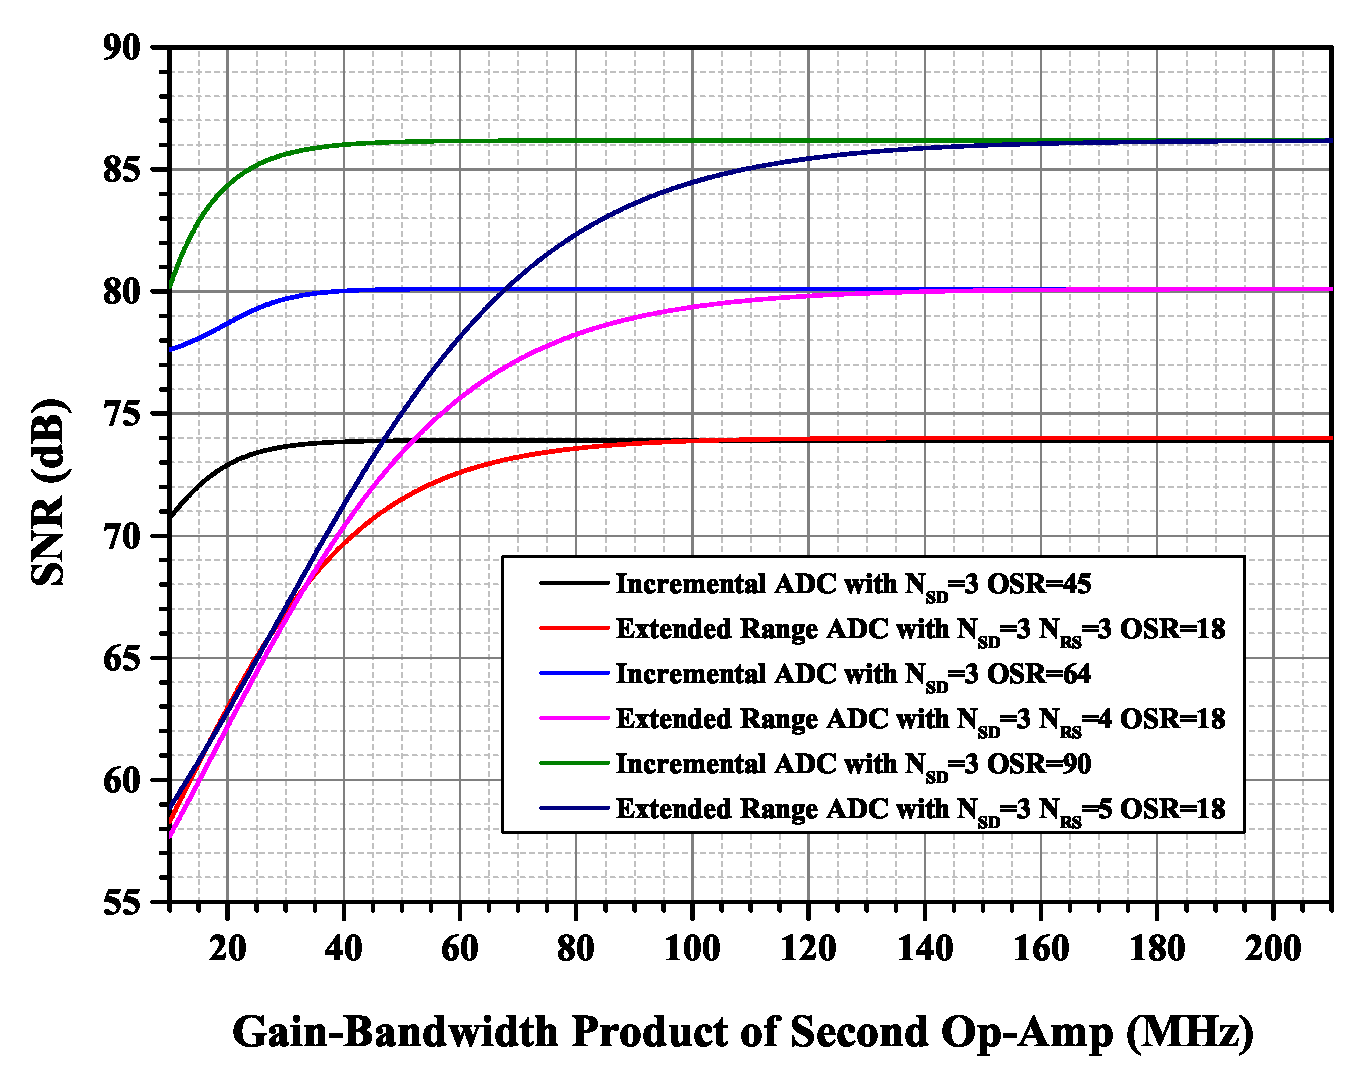
\includegraphics[width=2.5in]{Chap_paper01/Figures/SNR_GBW2_NSD3.eps}%
\label{SNR_GBW2_NSD3}}
\hfil
\subfloat[]{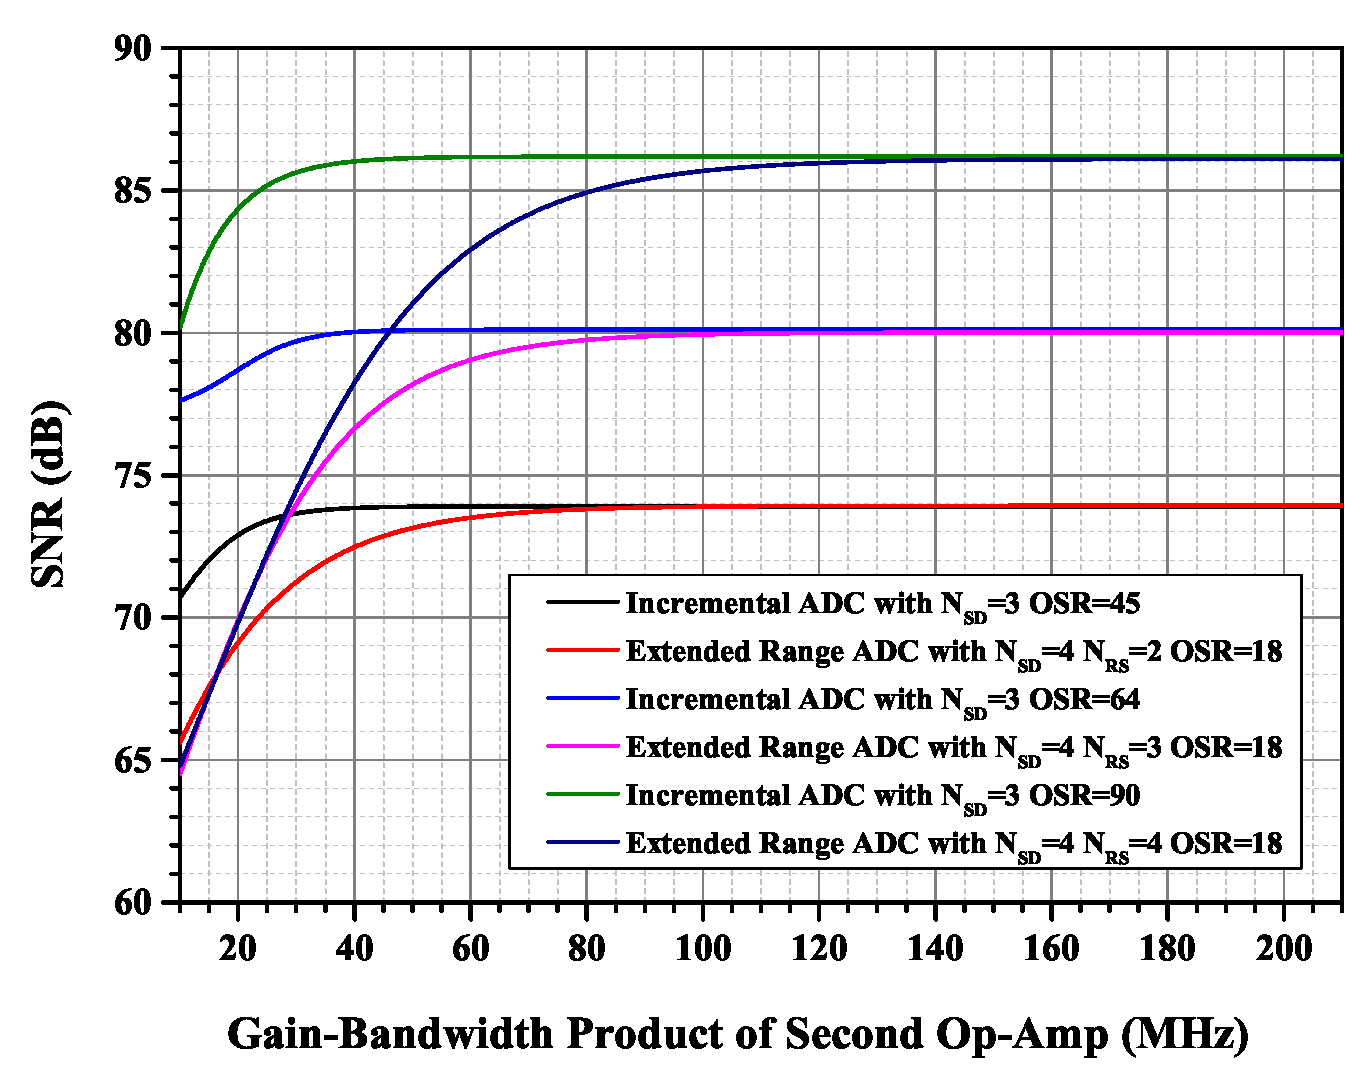
\includegraphics[width=2.5in]{Chap_paper01/Figures/SNR_GBW2_NSD4.eps}%
\label{SNR_GBW2_NSD4}}
\caption{Comparison of the IADC and extended-range IADC with different values of the second-integrator op-amp GBW}
\label{SNR_GBW2}
\end{figure}
\subsection{Performance Comparison}
The results of the analysis of the effect of op-amp gain and GBW on the ADC performance are summarized in the Tab.~\ref{COMPARISON}. Basically, it turns out that, by adding extended range to an IADCs, the strong reduction of the conversion time for the same ENOB is achieved at the expense of tougher op-amp gain and GBW specifications.
\begin{table}
\centering
\resizebox{\columnwidth}{!}{
\begin{tabular}{c|c|c|c|c|c|c|c|c|c}
\Xhline{3\arrayrulewidth}
\textbf{ENOB\textsubscript{TOT}} & \multicolumn{3}{c|}{\textbf{12}} & \multicolumn{3}{c|}{\textbf{13}} & \multicolumn{3}{c}{\textbf{14}} \\ \hline
\textbf{N\textsubscript{SD}} & 3 & 3 & 4 & 3 & 3 & 4 & 3 & 3 & 4 \\ \hline
\textbf{ENOB\textsubscript{INC}} & 12 & 9 & 10 & 13 & 9 & 10 & 14 & 9 & 10 \\ \hline
\textbf{N\textsubscript{RS}} & 0 & 3 & 2 & 0 & 4 & 3 & 0 & 5 & 4 \\ \hline
\textbf{OSR} & 45 & 18 & 18 & 64 & 18 & 18 & 90 & 18 & 18 \\ \hline
\textbf{Gain1 (dB)} & 36 & 58 & 50 & 38 & 76 & 70 & 40 & 80 & 80 \\ \hline
\textbf{Gain2 (dB)} & 36 & 58 & 52 & 38 & 74 & 60 & 40 & 80 & 70 \\ \hline
\textbf{GBW1 (MHz)} & 60 & 110 & 80 & 60 & 150 & 100 & 60 & 190 & 150 \\ \hline
\textbf{GBW2 (MHz)} & 40 & 90 & 80 & 40 & 130 & 90 & 40 & 160 & 130 \\ \Xhline{3\arrayrulewidth}
\end{tabular}
}
\caption{Comparison of the op-amp requirements for standalone IADC and extended-range IADC}
\label{COMPARISON}
\end{table}
The extended-range IADC with 3-bit quantizer and $N_{RS}=5$ requires 18 clock cycles per conversion to achieve 86~dB of SNR (14-bit ENOB). The same ENOB can also be achieved with 4-bit quantizer and $N_{RS}=4$ still requiring 18 clock cycles. However, it is clear that the sensitivity to op-amp non-idealities is different in the two cases. The ADC with $N_{RS}=5$ require a gain in both op-amps of 80~dB, a GBW in first-integrator op-amp of 190~MHz and a GBW in the second-integrator op-amp of 160~MHz, while the ADC with $N_{RS}=4$ requires more relaxed op-amp specifications (gain of 80~dB and GBW of 150~MHz, gain of 70~dB and GBW of 130~MHz in the two op-amps, respectively). This is due to the fact that a higher resolution in the ERADC requires higher accuracy in the residue value. However, the 4-bit IADC quantizer of the ADC with $N_{RS}=4$ is twice as large and power hungry than the 3-bit quantizer of the ADC with $N_{RS}=5$.

\section{Conclusion}

From the analysis and comparison carried out between the standalone IADC and the extended-range IADC explicitly turns out that, in order to attain a given SNR, the extended-range IADC requires a significantly lower number of clock cycles than a conventional IADC, but the requirements of the op-amps are much more stringent. Moreover, the partitioning of the resolution between IADC and ERADC in extended-range IADCs also affects the op-amp specifications: the higher is the resolution in the ERADC, the higher are the op-amp requirements.

